\section{Explainable Audit Alerts}\label{sec:explain}

A probability score by itself is not evidence an auditor can act on.
Opening or closing an investigation requires knowing \emph{why} a
transaction scored high and \emph{what}, concretely, is suspicious about
it -- ideally with a guarantee that the latter is not a plausible-sounding
story invented after the fact. Post-hoc graph-neural-network explainers
typically supply only an approximate, model-external account of that kind
\cite{wang2023reinforced}. The console instead attaches every alert a
fixed, two-layer explanation, both layers computed once per alert directly
from the persisted scoring bundle and the canonical transaction stream
(\texttt{src/modeling/alerts.py}): (1) exact per-feature attribution of the
score, tagged by feature family and glossed in plain English, and (2) graph
evidence obtained by literally replaying the transaction stream to the
alert's exact position in time, so that what the auditor is shown is
provably consistent with what the model saw rather than a post-hoc
rationalization. Every alert below is generated from each dataset's
persisted \texttt{final} bundle -- the offline, TGN-augmented research
champion -- not the deployed online scorer, which omits the TGN family
entirely (see the system section of this paper); the two are explicitly
distinguished throughout the paper.

\subsection{Layer 1: Family-Tagged TreeSHAP Attribution}
Attribution uses XGBoost's native \texttt{pred\_contribs} path, which runs
the exact TreeSHAP algorithm -- identical to the \texttt{shap} package's
\texttt{TreeExplainer} for tree ensembles \cite{lundberg2017unified,
lundberg2020local} -- as a pure tree traversal in margin space
\cite{chen2016xgboost}. Because attribution operates on the final boosted
tree ensemble, it is exact regardless of whether an input feature is a
hand-engineered topology statistic or a learned TGN embedding component
\cite{rossi2020temporal}; no approximation is introduced by mixing feature
provenances.

Each of the top-$n$ drivers returned for an alert is tagged with one of four
families: \texttt{ordinary} (amount, balance, category, prior-history),
\texttt{topology} (pure graph-shape statistics such as fan-in or
in-degree), \texttt{topology-amount-derived}, and \texttt{tgn}. The third
family exists because of an earlier finding in this paper: the lapping
detector's five columns (\texttt{cycle\_amount\_ratio},
\texttt{lap\_in\_recur}, \texttt{lap\_in\_payers}, \texttt{lap\_out\_recur},
\texttt{lap\_out\_payees}) are, on inspection, amount signal recovered
through a structural proxy rather than pure shape, so the alert layer
re-splits the bundle's coarser 13-column ``topology'' group (8 pure-structure
$+$ 5 amount-derived, out of 21/13/65, 8/13/65, 20/13/65 and 15/13/65
ordinary/topology/tgn columns for BankSim, IBM AML, SAP Würzburg and
synth\_erp respectively; \texttt{final\_champions.json}) at explanation time
so the two are never conflated in front of an auditor. Every driver also
carries a fixed plain-English gloss keyed off the feature name, e.g.\
\texttt{fan\_in} $\to$ ``distinct recent senders into the destination'',
\texttt{in\_cycle} $\to$ ``closes a money loop returning to its origin'', any
\texttt{lap\_*} column $\to$ ``recurrence of near-equal amounts (lapping
signature)'', and \texttt{tgn\_edge\_expectedness} $\to$ ``how expected this
sender$\to$receiver pair is to the learned temporal model (low = surprising)''.

The tagging surfaces real differences in what drives a score. BankSim's top
alert (score 0.9814) is led by \texttt{log\_amount} (SHAP $+3.35$,
\texttt{ordinary}), then \texttt{fan\_in}=49 (SHAP $+0.76$,
\texttt{topology}) and \texttt{dest\_in\_degree}=52 (SHAP $+0.63$,
\texttt{topology}). IBM AML's top alert (score 0.7283), by contrast, is led
by \texttt{lap\_out\_recur} (SHAP $+0.83$), explicitly tagged
\texttt{topology-amount-derived} rather than \texttt{topology} -- an honest
label that would be lost under a coarser ``graph feature'' bucket.

\subsection{Layer 2: Replay-Verified Graph Evidence}
The engine that computes topology features (\texttt{topology/engine.py})
persists per-transaction \emph{features} for every row, not the underlying
paths -- retaining a full cycle path for millions of transactions is not
worthwhile when only a handful will ever be shown to an auditor. The
evidence layer (\texttt{topology/paths.py}) instead replays the same
canonical edge stream, in the same order, with the same trailing window and
partition resets and the same node factorization as the streaming feature
pass, but only for the alerted transaction IDs. At each alerted transaction
it evicts stale window entries, \emph{reads} the graph state immediately
before insertion -- the identical as-of point the feature engine used -- and
only then inserts the edge. For a transaction closing a cycle, this yields
the full forward path (closing edge first, then the hops that complete the
loop) together with two derived quantities: \emph{amount conservation}
(the ratio of the smallest to largest hop amount around the loop) and
\emph{time span} (elapsed time from the earliest hop to the alerted
transaction). For a fan-in transaction, it yields the list of distinct
senders behind the destination within the trailing window, each with its
own amount and timestamp, most-recent first and capped at 25 for display.

This reconstruction is checked, not merely asserted: the replayed cycle
length must match the \texttt{cycle\_length} feature already stored for that
transaction by the batch pass; on any mismatch the alert reports the
discrepancy explicitly (``path not reconstructed'') rather than presenting an
unverified path. That invariant is what makes the evidence \emph{provably}
consistent with what the model saw, as opposed to a plausible narrative
constructed after the fact from correlated features. Two concrete examples
from IBM AML's alert set illustrate the range: alert 1 closes a 2-hop cycle
$5025 \to 1751 \to 5025$, conserving 10\% of the amount within 4 time units;
alert 4 closes a 5-hop cycle $7089 \to 9207 \to 7465 \to 9913 \to 9832 \to
7089$, conserving 100\% of the amount within 7 time units. BankSim's fifteen
fan-in alerts range from 6 to 63 distinct senders inside the window; the
seven highest-scoring cluster at 47--63 senders collecting into a single
merchant account -- a textbook mule-collection pattern.

The two layers are generated independently and can diverge revealingly.
Cycle-shaped features carry essentially zero gain importance model-wide on
three of the four datasets (BankSim, IBM AML, SAP Würzburg; synth\_erp is the
exception, and only marginally so), yet the replay still surfaces a
machine-verified closed cycle behind 8 of IBM AML's top-20 alerts and 6 of
synth\_erp's (\texttt{evidence\_type\_counts}, Table~\ref{tab:alert_precision})
-- because Layer 2 does not ask which features the model weighted, it asks
what structure actually exists around the flagged transaction. The two
layers answer different questions and neither substitutes for the other.

\begin{table}[t]
\centering
\caption{Top-$k$ audit-alert precision by dataset, test period, \texttt{final} champion bundle (\texttt{paper/data/alerts.json}).}
\label{tab:alert_precision}
\resizebox{\columnwidth}{!}{%
\begin{tabular}{lrrrrl}
\toprule
Dataset & Thresh. & $k$ & Fraud in top-$k$ & Prec.@$k$ & Evidence mix \\
\midrule
BankSim       & 0.4621 & 15 & 15/15 & \textbf{1.00} & fan\_in:15 \\
IBM AML       & 0.5162 & 20 & 20/20 & \textbf{1.00} & cycle:8, fan\_in:9, none:3 \\
SAP Würzburg  & 0.2566 & 10 & 2/10  & \textbf{0.20} & fan\_in:10 \\
synth\_erp    & 0.2388 & 20 & 20/20 & \textbf{1.00} & fan\_in:13, cycle:6, none:1 \\
\bottomrule
\end{tabular}}
\end{table}

%% FIGURE TODO: stacked horizontal bar chart, one bar per dataset, segments
%% = evidence_type_counts (fan_in / cycle / none) from alerts.json, annotated
%% with precision@k per dataset so the SAP Würzburg outlier is visually obvious
%% against the three datasets at 1.00.
\begin{figure}[t]
\centering
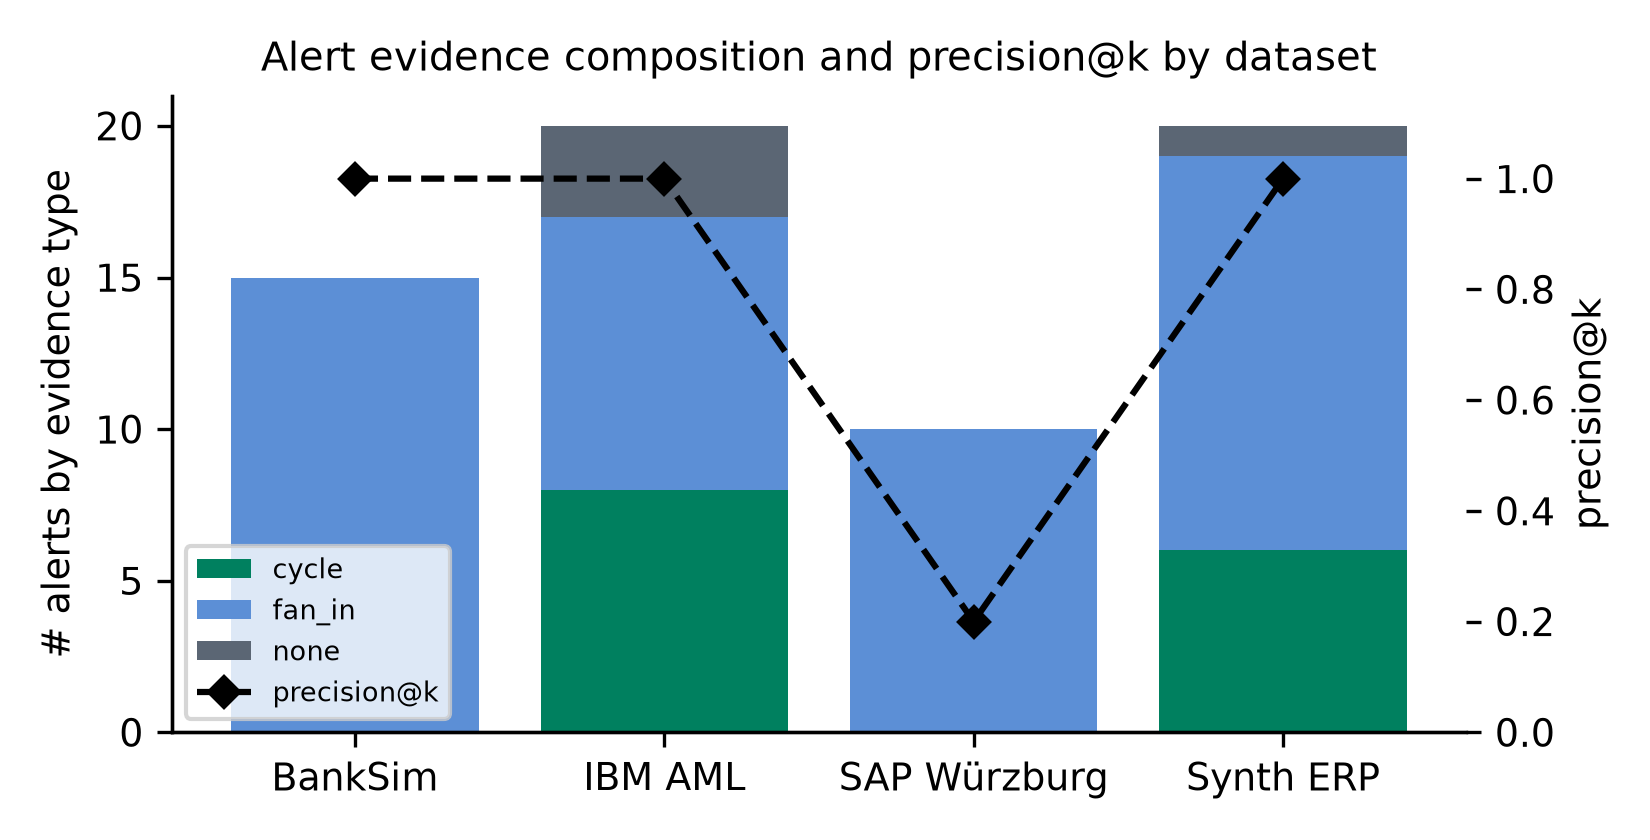
\includegraphics[width=\columnwidth]{figures/alert_evidence_mix.png}
\caption{Composition of graph evidence behind each dataset's top-$k$ alerts
(fan-in vs.\ cycle vs.\ no reconstructable structure), alongside precision@$k$.
Every bar sums to $k$ from Table~\ref{tab:alert_precision}.}
\label{fig:evidence_mix}
\end{figure}

\subsection{Per-Dataset Alert Precision}
Three of the four datasets reach perfect precision at their operating $k$
(Table~\ref{tab:alert_precision}): every one of BankSim's top 15, IBM AML's
top 20, and synth\_erp's top 20 test-period alerts is a labelled fraud. IBM
AML's 1.00 should not be over-read, however: its baseline model is already
saturated at $\mathrm{PR\text{-}AUC}\approx0.99$ (the ablation study reported earlier in this paper),
so a perfect top-$k$ here is consistent with the amount signal alone doing
the work and does not, on its own, demonstrate that topology mattered for
these particular alerts -- three of the twenty carry no reconstructable
fan-in or cycle evidence at all (\texttt{evidence\_type\_counts.none}=3),
meaning their risk drivers were purely \texttt{ordinary}/\texttt{tgn}.

SAP Würzburg is the outlier the ablation predicts: precision@10 is 0.20 (2 of
10), the weakest by a wide margin, the direct operational consequence of the
dataset's negative marginal structural lift reported elsewhere in this
paper, compounded by only 25 labelled test frauds. Every one of its ten
alerts is nonetheless a syntactically well-formed, replay-verified fan-in --
destinations collecting from 166 to 271 distinct senders in-window --
because those accounts are simply high-traffic general-ledger hubs
(\texttt{GL:895000}, \texttt{GL:300000}), not because fraud is present. This
is the clearest illustration in the paper of what Layer 2 actually
guarantees: the evidence is provably consistent with what the model saw,
never a guarantee that what the model saw was fraud. (Its test-partition
size also differs by source file: \texttt{final\_champions.json}, which
produced this bundle, reports 40{,}116 test rows / 25 frauds, while
\texttt{ablation.json}'s separately-run partition-aware split reports
40{,}139 -- the two pipeline runs are not the same split and should not be
merged.)

\subsection{Global Attribution Is Dataset-Specific, Not Universal}
Averaging $|\text{SHAP}|$ over a sample of each dataset's test rows
(\texttt{final\_champions.json}: \texttt{shap\_global\_top20}, 50{,}000
sampled rows for BankSim/IBM~AML/synth\_erp and the full 40{,}114-row test
partition for SAP Würzburg, since \texttt{bundle\_metadata.json} does not
itself carry per-feature magnitudes) shows that no single family dominates
across datasets (Table~\ref{tab:global_shap}).

\begin{table}[t]
\centering
\caption{Top-3 globally attributed features per dataset by mean $|$SHAP$|$ (margin space), with family tag (\texttt{paper/data/final\_champions.json}).}
\label{tab:global_shap}
\small
\begin{tabular}{lclr}
\toprule
Dataset & Rank & Feature (family) & Mean $|$SHAP$|$ \\
\midrule
\multirow{3}{*}{BankSim}
 & 1 & \texttt{category\_es\_transportation} (ordinary) & 0.675 \\
 & 2 & \texttt{fan\_in} (topology) & 0.609 \\
 & 3 & \texttt{dest\_in\_degree} (topology) & 0.558 \\
\midrule
\multirow{3}{*}{IBM AML}
 & 1 & \texttt{lap\_out\_recur} (topo.-amt-derived) & 0.588 \\
 & 2 & \texttt{log\_amount} (ordinary) & 0.296 \\
 & 3 & \texttt{lap\_out\_payees} (topo.-amt-derived) & 0.079 \\
\midrule
\multirow{3}{*}{SAP Würzburg}
 & 1 & \texttt{fan\_in} (topology) & 0.189 \\
 & 2 & \texttt{dest\_count\_prior} (ordinary) & 0.088 \\
 & 3 & \texttt{log\_amount} (ordinary) & 0.028 \\
\midrule
\multirow{3}{*}{synth\_erp}
 & 1 & \texttt{log\_amount} (ordinary) & 0.718 \\
 & 2 & \texttt{tgn\_edge\_expectedness} (tgn) & 0.407 \\
 & 3 & \texttt{dest\_in\_degree} (topology) & 0.357 \\
\bottomrule
\end{tabular}
\end{table}

BankSim's single most-attributed feature globally is a merchant-category
indicator, not a topology feature -- \texttt{fan\_in} and
\texttt{dest\_in\_degree} rank second and third -- even though BankSim is
the dataset with the strongest validated structural lift in this paper.
Amount and category signal dominates the average attribution even where
topology genuinely helps; the two findings are compatible because global
mean $|\text{SHAP}|$ and marginal ablation lift answer different questions
(which features move scores the most, vs.\ how much test-set PR-AUC a
feature group adds).

IBM AML's global top feature is \texttt{lap\_out\_recur}, tagged
\texttt{topology-amount-derived} rather than pure \texttt{topology} --
confirming at the dataset level the alert-level pattern noted above, and
consistent with \texttt{final\_champions.json}'s own recorded caveat for
this dataset (``baseline is amount-saturated ($\mathrm{PR\text{-}
AUC}\sim1.0$): margins here are uninformative''). No genuine cycle feature
appears in its top 20 at all, despite cycles accounting for 8 of its 20
alert-evidence blocks -- the model leans on the amount-derived lapping
proxy while Layer 2's independent replay still finds and shows a real
closed loop.

SAP Würzburg is the only dataset whose global top feature is a
\emph{pure} topology column (\texttt{fan\_in}), yet it also has the
negative marginal structural lift and the worst alert precision in this
paper: mean $|\text{SHAP}|$ measures how much a feature moves the score on
average, not whether that movement is correct, and \texttt{fan\_in} can be
the model's largest lever while remaining a poor discriminator when the
underlying counts reflect a handful of high-traffic GL hub accounts rather
than fraud. synth\_erp -- sanity/demonstration data, never thesis evidence --
shows a third pattern: \texttt{log\_amount} leads, with a learned TGN
feature and a topology feature close behind, echoing the earlier finding
that on this dataset learned and hand-engineered structure are
complementary rather than either dominating.

Together, Tables~\ref{tab:alert_precision} and~\ref{tab:global_shap} argue
against any single sentence like ``the model relies on graph structure'':
which family dominates, and whether that reliance is well-founded, is
dataset-specific. The console's honesty about that -- visible family tags,
replay-verifiable evidence, and a \texttt{ground\_truth\_label} kept for
research transparency but never surfaced to a real reviewer -- is the point
of the two-layer design, not a substitute for the ablation evidence that
grounds it.
